\documentclass[conference]{IEEEtran}
\IEEEoverridecommandlockouts
% The preceding line is only needed to identify funding in the first footnote. If that is unneeded, please comment it out.
\usepackage{cite}
\usepackage{amsmath,amssymb,amsfonts}
\usepackage{algorithmic}
\usepackage{graphicx}
\usepackage{textcomp}
\usepackage{xcolor}
\usepackage{url}
\def\BibTeX{{\rm B\kern-.05em{\sc i\kern-.025em b}\kern-.08em
    T\kern-.1667em\lower.7ex\hbox{E}\kern-.125emX}}
\begin{document}

\title{Exploring the factors and challenges in adopting GitHub Actions and its ecosystem\\}

\author{\IEEEauthorblockN{1\textsuperscript{st} Saif Sayed}
\IEEEauthorblockA{\textit{Department of Computer Science and Engineering} \\
\textit{University of Gothenburg}\\
Gothenburg, Sweden\\
gussayedfa@student.gu.se}
\and
\IEEEauthorblockN{2\textsuperscript{nd} Kardo Marof}
\IEEEauthorblockA{\textit{Department of Computer Science and Engineering} \\
\textit{University of Gothenburg}\\
Gothenburg, Sweden\\
gusmaroka@student.gu.se}
}

\maketitle

                                                                      %%% INTRODUCTION %%%
\section{Introduction}
    Continuous Integration (CI) has become an integrated part of collaborative software development awend DevOps practices. CI automates the quality of code checks, tests and integration of code changes in collaborative environments. The benefits of CI brings early detection of issues, fast feedback loops, increased code quality, reduced integration risks and continuous improvements. Famous examples of CI services include Jenkins, Travis, CircleCI and GitLab CI/CD \cite{dabbish2012social}. GitHub Actions (abbreviated as GHA) was introduced to the public in 2019 as an alternative CI service for GitHub repositories. GitHub introduced its marketplace for sharing automation tools in an effort for developers to reuse workflow components \cite{saroar2023developers}. \\ 

    The so called "Actions" refers to automated workflows triggered by specific events within a repository, including committing changes, opening pull requests, or creating new branches. These workflows streamline development processes by automating tasks and enhancing efficiency. GitHub's integration of GHA allows developers to define custom task sequences in response to events, simplifying collaboration and promoting a seamless development experience \cite{chandrasekara2021getting}. \\



    The growing popularity of GHA is immense, with on average more than 20 million GitHub Action minutes used per day in 2023. This growth leads to a 169\% increase in the usage of automating tasks in public projects,  pipelines and more\cite{github2023octoverse}. Given its popularity,  the increasing usage of GHA has lead to an emergence of its own ecosystem \cite{decan2022use}.  According to Decan et al. \cite{decan2022use}, the growing ecosystem of GHA bears similarities to reusable software libraries distributed by package managers such as npm, Cargo, RubyGems, Maven and PyPI among others. Where these ecosystems are well known to suffer from variety of issues such as obsolescence, dependency issues, breaking changes and security vulnerabilities to name a few\cite{decan2022use}. The authors go on to state "\textit{The GHA ecosystem is likely to suffer from very similar issues and these issues will continue to become more important and more impactful, as the number of reusable Actions continues to grow at a rapid pace.}"\\

    Given the concerns surrounding the GHA ecosystem, it is self-evident that developers will experience the effects of these issues.  Moreover, it's worth noting that not all Actions are available on the GitHub marketplace. Many developers create and maintain their own Actions within local repositories, without making them available on the marketplace. The authors  conducted an analysis of prevalent automation practices on GitHub and discovered that 43.9\% of repositories in their dataset reflected this behavior \cite{decan2022use}.\\

    Due to its novelty, there is limited understanding of the challenges faced when implementing GHA.  
    Therefore,  by systematically analysing StackOverflow posts, GitHub Discussions threads, tags, and other pertinent repositories, alongside the utilisation of database queries and APIs, we aim to quantitatively examine the questions, topics, and answers surrounding GHA. This endeavor not only facilitates the clarification of prevalent issues but also provides insights into potential solutions and areas requiring further research and development within the GHA landscape.\\

    Through this research, we intend to answer the following questions:\\


    \textbf{RQ1: What factors cause developers to rely on Local Actions within their repositories, as opposed to utilizing Actions available on the GitHub Marketplace?}\\

    Both Saroar et al. \cite{saroar2023developers} and Decan et al. \cite{decan2022use} observed that many repositories still prefer to use Local Actions within their repositories, despite the availability of numerous open-source and reusable Actions on the GitHub Marketplace. However, these studies do not investigate the exact factors or make comparisons between the two types of Actions that contribute to developers' preferences. We selected RQ1 to distinguish the problems faced between locally maintained and Marketplace Actions and reach a conclusion. Additionally, some workflows utilize both types of actions, and understanding which types are more commonly locally maintained can provide valuable insights into the decision-making process for designing and developing workflows. \\

 \textbf{RQ2: In what ways do the key issues encountered in GHA parallel those found in other software ecosystems?}\\

    This research question is inspired by the concerns raised by Decan \cite{decan2022use}, as previously mentioned. The objective is to compile a list of current issues prevalent in reusable software libraries distributed via package managers and draw parallels with our research findings. This comparative analysis aims to determine whether these concerns are indeed applicable to the GHA ecosystem. If similarities are found, it will aid in identifying effective solutions previously implemented in other ecosystems to address these issues. Subsequently, these solutions can be adapted for the GHA ecosystem to prevent the escalation of such problems in the future.



                                                                        %%% RELATED WORK %%%

\section{Related Work}
    After just 18 months since its official release, previous research has demonstrated a notable surge in the popularity of GHA, leading to a gradual shift away from conventional CI/CD services in GitHub repositories \cite{golzadeh2021rise}. Unlike conventional CI/CD services, GHA assists the software development processes by improving code reviews, team communication and internal repository management in addition to automating the build and test procedures of software \cite{chandrasekara2021hands}. As previously mentioned, this emerging popularity on the use of GHA and the increasing number of reusable Actions that can be found on its marketplace led GHA to be considered similar to popular reusable software libraries distributed by package managers such as npm, Cargo, RubyGems, Maven and PyPI and so on. However, this also means GHA is more likely to face similar problems that are currently encountered by these reusable libraries \cite{decan2022use}. Consequently, this would increase the chances of failure when building GitHub workflows in GitHub repositories leading to unsuccessful deployment of software packages. \\

    According to Decan \cite{decan2022use}, the GHA ecosystem deserves to be studied as all other reusable software ecosystems that have made progress in finding issues related to them. Since GHA is a new emerging ecosystem, there is a lack of research and studies that have been carried out to identify the challenges and issues that are encountered in GHA. The authors point out that the GHA ecosystem is exposed to similar challenges, such as obsolescence \cite{decan2018evolution} \cite{cogo2021deprecation}, dependency issues \cite{decan2019empirical} \cite{soto2021comprehensive} \cite{decan2019package}, breaking changes \cite{dietrich2019dependency}\cite{decan2018impact} and security vulnerabilities \cite{zimmermann2019small} \cite{kula2018developers}, that are encountered in well-researched ecosystems. This section aims to briefly describe some of the issues pointed out above, using findings from related literatures, that are likely to appear in GHA.

    \subsection{Obsolescence}
        Software codes are regularly updated to add features, fix bugs, etc. Sometimes functions or parts of code become deprecated meaning they are outdated and no longer used; this usually happens after a long period of time, when parts of the software code are replaced by an improved version. Generally, it is a good practice to avoid using deprecated code. Through the findings of Cogo et al. \cite{cogo2021deprecation}, deprecated code used in npm packages has shown to give rise to risks such as incompatibility between two different dependant libraries, presence/absence of features, bugs, security vulnerability and more. Cox et al. \cite{cox2015measuring} found that deprecated systems are four times more likely to suffer from security issues and backward incompatibilities than systems that are up-to-date. In the context of GHA, there is a high possibility that a significant amount of code used within the workflow is deprecated which may consequently lead to build failures.

    \subsection{Dependency Issues}
        Software systems are usually developed using pre-existing and reusable packages such as modules, components, libraries, etc \cite{decan2019empirical}\cite{soto2021comprehensive}. Consequently, this leads to a large extent of dependencies between the reused packages and the original software code. According to Dietrich et al. \cite{dietrich2019dependency}, software developers struggle to choose which versions of a given package to use and that a handful number of software systems encounter runtime version conflicts due to incompatibility with the versions of other dependant packages. Actions and workflows that depend on jobs from other Actions might fall on a similar pitfall of runtime version conflicts and possibly other dependency issues. Valenzuela-Toledo and Bergel \cite{valenzuela2022evolution} claim they have found instances of workflows where modifications were made to update the version of the tool/software being used in a particular job (e.g., Figure 1 \cite{valenzuela2022evolution}  ).

\begin{figure} [h]
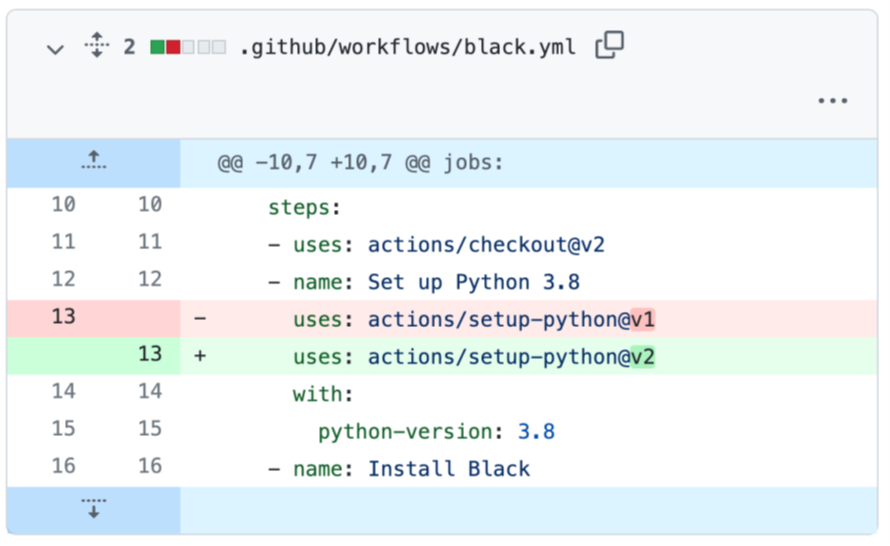
\includegraphics[width=0.5\textwidth]{Figure 1.png}
\caption{Modifying python version \cite{valenzuela2022evolution} }
\end{figure}

    \subsection{Security Vulnerabilities}
        Software that depends on open source and free reusable libraries provided by package managers like npm are more likely to be exposed to security vulnerabilities. To quote Zimmermann et al. \cite{zimmermann2019small}, they mention the following: \\

        \textit{"The open nature of npm has boosted its growth, providing over 800,000 free and reusable software packages. Unfortunately, this open nature also causes security risks, as evidenced by recent incidents of single packages that broke or attacked software running on millions of computers.”} \\

        According to Koishybayev et al. \cite{koishybayev2022characterizing}, one example of a similar attack using the GHA ecosystem is to perform deployments based on the attacker’s code by triggering a misconfigured workflow through a new pull request. Since GHA consists of many open-source reusable Actions, workflow and GHA developers need to be extra careful on choosing what packages they depend on for building jobs. It is a good practice to depend on first-party packages and packages from trustworthy maintainers \cite{zimmermann2019small}. \\

        Saroar et al. \cite{saroar2023developers} mentions that even though the GHA platform provides a marketplace for sharing and reusing open-source Actions, there are still many repositories that prefer to maintain their own GHA locally within their repositories. The survey analysis conducted by the authors revealed some challenges GitHub users face using the Marketplace where 7 out of 25 participants found it difficult to search for products and hard to check product quality (see Figure 2). Saroar et al. \cite{saroar2023developers} quotes one of the participants from the survey: \\

\textit{"Marketplace does not provide an effective way to filter and sort based on quality, version, contributions, etc."}\\

\begin{figure} [h]
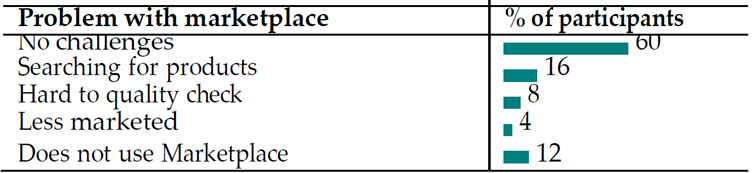
\includegraphics[width=0.5\textwidth]{Table 1.png}
\caption{Challenges found when using GitHub Marketplace \cite{saroar2023developers} }
\end{figure}

	Decan et al. \cite{decan2022use} raised concerns regarding potential issues that might be encountered by GHA, including obsolescence \cite{decan2018evolution} \cite{cogo2021deprecation}, dependency issues \cite{decan2019empirical} \cite{soto2021comprehensive} \cite{decan2019package}, breaking changes \cite{dietrich2019dependency} \cite{decan2018impact}, and security vulnerabilities \cite{zimmermann2019small} \cite{kula2018developers}. These issues have already been faced in reusable software libraries within well-researched ecosystems. In our exploratory study, we aim to investigate whether similar problems also exist within the GHA ecosystem. Moreover, we will compile a list of specific issues from the aforementioned papers and compare our research findings on key issues in GHA with those identified in other ecosystems discussed in the literature. By doing so, we can potentially identify solutions proposed for similar issues in other ecosystems, which could offer insights into addressing the challenges encountered in GHA.\\

	Furthermore, our study aims to build upon the findings of Saroar et al. \cite{saroar2023developers}, providing explanation for their observations regarding the distribution of Local Actions compared to Actions from the marketplace. While the survey conducted by the authors offers valuable insights into the challenges faced when utilizing the GitHub Marketplace, it lacks comprehensive research and comparison involving Local Actions. The primary objective of our research is to evaluate repositories' preferences in utilizing Local Actions versus actions from the GitHub Marketplace. By doing so, we aim to identify and explain the factors that contribute to these preferences and the resulting differences in adoption.



                                                                        %%% RESEARCH MOTHODOLOGY %%%

\section{Research Methodology}
    With this study we aim to answer some of the challenges developers face when building GHA. Our goal is to evaluate whether similar challenges and issues from well-researched reusable libraries can be spotted in the GHA ecosystem.\\

    In this section, we describe the research questions we are trying to answer and the research strategies which will be implemented to facilitate our explorative study. Additionally, we would like to emphasize that we are employing a mixed method study, utilising different data collection and analysis methods that will be described and motivated after each research question. Finally, we identify and explain the limitations relevant to our research.

    \subsection{Research questions and methodology}
        \textbf{RQ1: What factors developers to rely on locally maintained Actions within their repositories, as opposed to utilising Actions available on the GitHub marketplace?}
        \\

        \textbf{Research Method:}  Repository Mining \\
          This research question is answered by measuring similar characteristics of GitHub repositories that utilise GHA. And how these characteristics can correlate with the usage of locally maintained Actions (Local Actions). By quantitatively measuring the following characteristics, we can make an argument for whether or not the preference for using Local Actions can be tied to project size, project complexity, organization, and team size. \\
          \begin{itemize}
            \item \textbf{Repository size:} Repository size in bytes. This includes all files such as source code, artifacts, documentation, data, etc.
            \item \textbf{Number of contributors:} How many developers have contributed to the repository. May indicate the size of the team working on the project.
            \item	\textbf{Number of programming languages used:} How many types of programming langugaes used within the project. May indicate a higher complexity of the project.
            \item \textbf{Date of repository creation:} Date of creation. May indicate trends and cultral shifts.\\
            \item \textbf{Size of source code:} Only the amount of source code available in bytes. May also indicate a higher complexity of the project. \\
          \end{itemize}
          
          \subsubsection{\textbf{Data Collection}}
            The study utilizes python scripts\footnote{https://github.com/WalrusArtist/SEM-Thesis/tree/kardo/python} to collect and store repositories using GHA. Workflow files are fetched from all the stored GitHub repositories using the GitHub API.  The workflow files are then parsed, with each line iterated, to search for the $uses:$ keyword and check whether the reference of the Action matches that of a Marketplace Action or a Local Action. To distinguish between the patterns, we check whether the Action reference matches the pattern $/.github*$ or $*.yml$ or $*.yaml$. If it does, we determine that it is a Local Action, due to the reason that Local Actions are called from a file path that reside within the $/.github*$ folder or end with the file extention $*.yml$ or $*.yaml$.
            \\ Similarly, for Marketplace Actions we check whether the Action reference contains the symbol $@$. If it does, we can determine that it is a Marketplace Action. \\ However, an important note here is that developers and organizations may have references of Actions that are locally maintained by themselves, but the Actions are kept in other repositories. In this case, an $@$ symbol is also present. To fully determine if an Action is indeed from not locally maintained, we have applied a step to verify that the owner of the repository and the owner of the Action do not match. The owner verification step can help with the accuracy of the measurement, because in certain cases the pattern in which the Action is called can be nuanced and can lead to false positives in measuring the amount of Marketplace Actions\\ 
            To avoid redundancy, whenever an Action name is parsed out, that record is saved into a set with an attribute called $times.used$. If the same action is referenced elsewhere in Workflow, we increase $times.used$ by one data point. The $times.used$ attribute can allow us to measure the resuability of an Action within a repository workflow.\\

          \subsubsection{\textbf{Data Analysis}}
            In the analysis we have taken a quantitative approach to measure the correlations between repository characteristics and the number of Actions. In order to ensure an accurate understanding of what factors are correlated to relying on Local Actions more, the same quantitative analysis has been conducted for both Local and Marketplace Actions. We have used the Spearman correlation coefficient (PCC) method to measure the correlations coefficient of each of the repository characteristics alongside the number of Local and Marketplace Actions available and referenced. The Spearman rank correlation coefficient, \(\rho\), is a measure of the strength and direction of the association between two ranked variables. It is calculated using the formula:

            \begin{equation}
            \rho = 1 - \frac{6 \sum d_i^2}{n(n^2 - 1)}
            \end{equation}
            
            where \(d_i\) is the difference between the ranks of each pair of observations and \(n\) is the number of observations. This non-parametric measure is used to assess how well the relationship between two variables can be described using a monotonic function. \\             
            \\ We have then compared the results of these measurements to indicate if the preference for selecting Local Actions increases more than Marketplace Actions alongside any of the repository characteristics. \\
            Owner based frequency measurement for the amount of Local Actions available per owner can also help with determining whether big organizations lean more towards developing in-house Actions. For this analysis we have aggregated the results of Local Actions available per repository and categorized them per owner. The results from this analysis can indicate whether bigger organizations have a higher frequency in utilizing Local Actions more. \\

        \textbf{RQ2: In what ways do the key issues encountered in GHA parallel those found in other software ecosystems?}\\

            \textbf{Research Method:} Repository Mining\\
            We are already aware of the problems encountered in other ecosystems. Our goal is to identify similar challenges and/or issues within the GHA ecosystem and evaluate the impact of these problems.\\
            To address RQ2, we plan to carry out repository mining. Through repository mining, we can collect vast amounts of data from relevant software repositories using GHA. We can also automate the process of mining data by developing scripts\footnote{https://github.com/WalrusArtist/SEM-Thesis/tree/kardo/python}  and easing the process of going through multiple repositories \cite{chaturvedi2013tools}.\\

            \subsubsection{\textbf{Data Collection}}
                Repository mining is conducted by utilizing APIs and database queries to collect relevant data from Stack Overflow, GitHub Discussions, and other pertinent repositories. To collect data from GitHub discussions, we utilize GraphQL API  in our scripts\footnote{https://github.com/WalrusArtist/SEM-Thesis/tree/kardo/python} to extract and store relevant discussion posts in JSON format. Particularly, we search for all the discussion posts that contain the query string $GitHub Actions$ . Then, the scripts target the following keywords and their synonyms to gather posts that may contain the following relevant problems: \\

              \begin{itemize}
                \item \textbf{Obsolescence:} Outdated, Legacy, Deprecat, Phasing out, Obsolete, Unmaintained
                \item \textbf{Dependency issues:} Dependency, conflict, mismatch, Package, Version, Dependency problem, Incompatible dependenc
                \item	\textbf{Breaking changes:} version, incompatible, API changes, Breaking updates, Breaking modifications, Breaking alterations, Disruptive changes
                        \item \textbf{Security vulnerabilities:} security, Security flaws, Security risk, Vulnerabilities, Exploit, loopholes, Attack\\
              \end{itemize}
                A similar approach is used to collect questions from Stackoverflow using the Stackoverflow API. Our scripts searches for all the questions that are tagged $GitHub-Actions$ and then targets the aforementioned issues and their synonyms. The discussion posts and questions will be analyzed manually, and conclusions about the problems will be drawn.\\

            \subsubsection{\textbf{Data Analysis}}
                In our data analysis approach, we employed repository mining techniques to analyze patterns and trends in StackOverflow posts, GitHub Discussions threads, and repository data obtained through APIs and database queries. Quantitative analysis encompassed descriptive statistics such as visualization methods including heatmaps. For qualitative analysis, our first step was to compile issues from other existing literature and group them into four themes: i) Obsolescence, ii) Dependency issues, iii) Breaking changes, and iv) Security vulnerabilities. Our collected dataset through MSR was already grouped into these themes during data collection where the data was filtered based on the synonyms appearning in the discussion or stackoverflow threads. However, there were cases when we had to map the same issue to more than one theme. The reason behind this overlapping is because of the close relation and dependency between these themes. For instance, there might be an issue related to security that is a consequence of depending on outdated software packages; in this case the same issue can be grouped to each of these themes 'Obsolescence', 'Dependency Issues', and 'Security vulnerabilities'. \\
                In our second step of our qualitative analysis, we utilized open coding to divide our collected issues in each theme to identify further relevant sub-themes which captures more than one synonym and labelled the issues using a list of synonym terms that appears on the sub-themes. We found that the posts that contain more than one term from the synonyms were more relevant to the theme. Then, we utilized axial coding to find patterns and relation between the themes. For instance, if a specific issue from a particular theme is also relevant to other themes,  we added the related theme to the list of synonyms labelling the relation between one or two themes. Our thematic coding is visually presented in Table 1.\\
                In summary, our qualitative analysis contained four main themes labelled with the keywords  'Obsolescence', 'Dependency Issues', and 'Security vulnerabilities' and smaller sub-themes labelled with a list of synonyms and related themes. An example of such a list would be $['Outdated', 'Legacy', 'Dependency Issues' ]$. Overall, our approach aimed to provide a comprehensive understanding of the challenges in the GHA ecosystem parallel to other software ecosystems.\\
\begin{tabular}{|c|c|}
  \hline
  \textbf{Main themes} & \textbf{Sub-themes} \\
  \hline
  \hline
    Security Vulnerabilities & Cell 2  \\
  \hline
   Dependency changes & Cell 6 \\
  \hline
  \hline
   Obsolescence & Cell 6 \\
  \hline
  \hline
   Breaking Changes & Cell 6 \\
  \hline
\end{tabular}

        These methods ensure a systematic approach to address each research question effectively.\\


    \subsection{Threats to Validity}
        In this section, we discuss the limitations and threats to
        validity and how we can mitigate them.\\

        \textbf{External Validity:} Since our repository mining procedure is supposed to collect data from diverse GitHub repositories with different implementation of workflows, programming languages and size of the project, the results we obtain might differ depending on these factors and our findings can not be generalized for all types of GitHub projects. However, it is possible to group the projects based on their size, programming language, etc. After grouping the projects, we could try to analyse data from each group and identify a common trend between the results to generalize our findings.\\

	\textbf{Construct Validity:} The questionnaire, we are planning to use as our survey instrumentation, might have errors or inconsistencies. The formulated questions might be unclear, ambiguous and/or irrelevant. We could address this risk by adhering to a well-defined criterion for formulating questionnaires. Additionally, we could conduct pilot testing to validate our survey instrument.\\

        \textbf{Response bias:} Collecting data through online surveys carries some risks and may result in anomalies in our results. Specifically, distributing surveys via social media can lead to invalid responses, and we may also face challenges in obtaining a sufficient number of responses to draw meaningful conclusions. To mitigate these potential limitations, we can consider distributing surveys through highly maintained development platforms or reaching out to potential companies in person. 

							    	      %%%RESULTS%%%

\section{Results}

  \subsection{RQ1}
      For RQ1, after collecting data across 4166 GitHub repositories that were on the top one-thousand list of popular repositories for the years throughout 2020, 2021, 2022, 2023 and 2024, we applied a filter to dismiss repositories that did not use any Actions. The number of repositries reduced to 1754. \\ 
      In these repositories, Marketplace Actions consisted of 92.64\% of the total Actions, while the remaining 7.36\% consisted of Local Actions. And when analysing the number of times each Action was referenced in other parts of the workflow, we found that the result was quite similar with 92.62\% for Marketplace Actions and 7.38\% for Local Actions. 
      \\
      Data on number of different programming languages, repository size, number of contributors, date of repository creation and bytes of source code were also collected in order to see if there were any correlations between these repository attributes and the amount of Marketplace or Local Actions used or referenced.
      Table \ref{tab:correlation_results} demonstrates the results of the correlations, categorized as Marketplace Actions and Local Actions. The number of elements in set $N$ is denoted by $|N|$, similarly for set $M$. \\
      
      \begin{table}[h]
          \centering
          \caption{Spearman Correlation Coefficients between Repository Characteristics and GitHub Actions}
          \label{tab:correlation_results}
          \hspace{-1cm}
          \begin{tabular}{|l|l|r|}
              \hline
              \textbf{Repository Characteristic} & \textbf{GitHub Action Type} & \textbf{(\(\rho\))} \\
              \hline
              Source Code size (bytes) & $|M|$ Local Actions & 0.23 \\
              \hline
              $|N|$ contributors &  $|M|$ Local Actions & 0.21 \\
              \hline
              Repo created (Unix timestamp) &  $|M|$ Local Actions & -0.11 \\
              \hline
              $|N|$ programming languages & $|M|$ Local Actions & 0.16 \\
              \hline
              Repository size (bytes) & $|M|$ Local Actions & 0.20 \\
              \hline
              Source Code size (bytes) & $|M|$ Local Actions referenced & 0.24 \\
              \hline
              $|N|$ contributors  & $|M|$ Local Actions referenced & 0.17 \\
              \hline
              Repo created (Unix timestamp) & $|M|$ Local Actions referenced & -0.14 \\
              \hline
              $|N|$ programming languages & $|M|$ Local Actions referenced & 0.23 \\
              \hline
              Repository size (bytes) & $|M|$ Local Actions referenced & 0.21 \\
              \hline
              Source Code size (bytes) & $|M|$ Marketplace Actions & 0.33 \\
              \hline
              $|N|$ contributors & $|M|$ Marketplace Actions & 0.30 \\
              \hline
              Repo created (Unix timestamp) & $|M|$ Marketplace Actions & -0.10 \\
              \hline
              $|N|$ programming languages & $|M|$ Marketplace Actions & 0.38 \\
              \hline
              Repository size (bytes) & $|M|$ Marketplace Actions & 0.27 \\
              \hline
              Source Code size (bytes) & $|M|$ Marketplace Actions referenced & 0.40 \\
              \hline
              $|N|$ contributors & $|M|$ Marketplace Actions referenced & 0.37 \\
              \hline
              Repo created (Unix timestamp) & $|M|$ Marketplace Actions referenced & -0.17 \\
              \hline
              $|N|$ programming languages & $|M|$ Marketplace Actions referenced & 0.41 \\
              \hline
              Repository size (bytes) & $|M|$ Marketplace Actions referenced & 0.30 \\
              \hline
          \end{tabular}
      \end{table}
      
      \subsection{Analysis of Correlations}
      
      \subsubsection{Local Actions}
      For Local Actions, several repository characteristics showed weak positive correlations:
      
      \begin{itemize}
          \item \textbf{Source Code Size:} A weak positive correlation (\(\rho = 0.23\)) was observed between the source code size and the number of Local Actions. This suggests that repositories with larger codebases tend to use more Local Actions.
          \item \textbf{Number of Contributors:} A weak positive correlation (\(\rho = 0.21\)) indicates that repositories with more contributors are slightly more likely to use Local Actions.
          \item \textbf{Repository Size:} Similar to the source code size, a weak positive correlation (\(\rho = 0.20\)) was found, reinforcing the idea that larger repositories are slightly more likely to utilise Local Actions.
          \item \textbf{Number of Programming Languages:} There is a weak positive correlation (\(\rho = 0.16\)), implying that repositories with a higher number of programming languages tend to use more Local Actions.
          \item \textbf{Repository Creation Date:} A weak negative correlation (\(\rho = -0.11\)) was observed, indicating that older repositories are less likely to use Local Actions.
      \end{itemize}
      
      \subsubsection{Marketplace Actions}
      Marketplace actions showed generally stronger correlations with repository characteristics compared to Local Actions:
      
      \begin{itemize}
          \item \textbf{Source Code Size:} There is a weak positive correlation (\(\rho = 0.33\)) between the source code size and the use of Marketplace Actions, indicating that larger codebases are more inclined to use Marketplace Actions.
          \item \textbf{Number of Contributors:} A weak positive correlation (\(\rho = 0.30\)) suggests that repositories with more contributors are more likely to use Marketplace Actions.
          \item \textbf{Repository Size:} A similar trend is observed with a weak positive correlation (\(\rho = 0.27\)), suggesting that larger repositories favor Marketplace Actions.
          \item \textbf{Number of Programming Languages:} The strongest positive correlation (\(\rho = 0.38\)) among all characteristics was found here, indicating a significant tendency for repositories with more programming languages to use Marketplace Actions.
          \item \textbf{Repository Creation Date:} A weak negative correlation (\(\rho = -0.10\)) indicates that older repositories are slightly less likely to use Marketplace Actions.
      \end{itemize}
      
      \subsubsection{Referenced Actions}
      When considering Actions referenced within repositories:
      
      \begin{itemize}
          \item \textbf{Local Actions Referenced:} The correlation coefficients for referenced Local Actions are slightly higher compared to non-referenced ones, with the highest being source code size (\(\rho = 0.24\)) and number of programming languages (\(\rho = 0.23\)).
          \item \textbf{Marketplace Actions Referenced:} The correlations are generally higher for Marketplace Actions referenced, with the number of programming languages showing a moderate positive correlation (\(\rho = 0.41\)) and source code size (\(\rho = 0.40\)).
      \end{itemize}

      \subsubsection{Organizational Usage of Local Actions}

      In addition to the correlation analysis, we examined the usage of Local Actions by various organizations. Table \ref{tab:org_usage} lists the top organizations based on their use of Local Actions. Notably, large organizations such as HashiCorp, Google, Microsoft, and Facebook are prominent in the usage of Local Actions, indicating a preference for maintaining their own workflows rather than relying solely on marketplace actions.
      
      \begin{table}[h]
          \centering
          \caption{Top Organizations by Use of Local Actions}
          \label{tab:org_usage}
          \begin{tabular}{|l|c|}
              \hline
              \textbf{Organization} & \textbf{Number of Local Actions} \\
              \hline
              HashiCorp & 58 \\
              Datafuselabs & 46 \\
              Hugging Face & 39 \\
              NovuHQ & 26 \\
              External Secrets & 26 \\
              Google & 25 \\
              Backstage & 25 \\
              Grafana & 23 \\
              KubeVela & 22 \\
              Earthly & 20 \\
              Cilium & 19 \\
              LanceDB & 19 \\
              Firezone & 18 \\
              ZenML-io & 17 \\
              Calcom & 17 \\
              Coqui AI & 15 \\
              Microsoft & 14 \\
              Web Infra Dev & 14 \\
              Appsmithorg & 14 \\
              Anchore & 13 \\
              Rustic-rs & 13 \\
              LibJXL & 13 \\
              Anuraghazra & 12 \\
              Vercel & 12 \\
              Haiibo & 12 \\
              Bitnami & 11 \\
              Chroma Core & 11 \\
              MartinVonz & 11 \\
              DataDog & 11 \\
              Apache & 11 \\
              Kafbat & 10 \\
              Lienol & 10 \\
              Mandiant & 10 \\
              Argilla-io & 10 \\
              CloudQuery & 10 \\
              OpenTofu & 10 \\
              Alibaba & 9 \\
              Keiyoushi & 9 \\
              Sigstore & 9 \\
              DeterminateSystems & 9 \\
              Kiddin9 & 9 \\
              RustDesk & 9 \\
              Techno Tim & 9 \\
              Facebook & 9 \\
              Lucidrains & 9 \\
              Zitadel & 9 \\
              JupyterLite & 8 \\
              \hline
          \end{tabular}
      \end{table}
      
      The predominance of large organizations in the use of Local Actions may be attributed to concerns over security risks and dependency issues associated with marketplace actions. Larger organizations might prefer to maintain control over their workflows to mitigate potential vulnerabilities and ensure stability. However, further investigation is needed to substantiate these claims and understand the underlying reasons behind this trend.
      
      \subsection{Discussion}
      The results indicate that certain repository characteristics, such as source code size, number of contributors, and number of programming languages, are positively correlated with the usage of GitHub Actions, whether locally maintained or from the marketplace. The stronger correlations for Marketplace Actions suggest that repositories with more complexity and collaboration tend to leverage Marketplace Actions more frequently. Conversely, the weak negative correlations with repository creation date suggest that newer repositories are more inclined to adopt both types of actions, potentially reflecting evolving practices and the increasing availability of GitHub Actions over time.
      
      In conclusion, the analysis provides insights into how various repository characteristics influence the adoption and referencing of GitHub Actions, highlighting trends that could inform best practices for repository management and automation strategy.
    


  \subsection{RQ2}
    For RQ2, we have found three of four themes that have issues from GHA that can be mapped to issues from other ecosystems. The theme that showed the highest number of mapped issue in GHA was 'Security Vulnerability'. Following this theme were the themes 'Dependency changes' and 'Obsolescence'  that had almost the same number of mapped issue. However, our reasearch work did not find similar issues in GHA that can be mapped for the theme 'Breaking changes'. Figure 3 and 4 shows a heatmap of the issues found in each of the themes in GitHub Discussions and Stackoverflow before mapping the data. Figure 5 and 6 shows a heatmap of the issues found in each of the themes  in GitHub Discussions and Stackoverflow after mapping the data.

    \begin{minipage}{\linewidth}
      \begin{tabular}{|c|c|}
        \hline
        \multicolumn{2}{|c|}{\textbf{Security Vulnerability}} \\ \hline
        \textbf{Other Ecosystems} & \textbf{GHA} \\
        \hline
        \hline
        Cell 1 & Cell 2  \\
        \hline
        Cell 3 & Cell 6 \\
        \hline
      \end{tabular}
      \end{minipage}
      
      \begin{minipage}{\linewidth}
      \begin{tabular}{|c|c|}
        \hline
        \multicolumn{2}{|c|}{\textbf{Obsolescence}} \\ \hline
        \textbf{Other Ecosystems} & \textbf{GHA} \\
        \hline
        \hline
        Cell 1 & Cell 2  \\
        \hline
        Cell 2 & Cell 6 \\
        \hline
      \end{tabular}
      \end{minipage}
      
      \begin{minipage}{\linewidth}
      \begin{tabular}{|c|c|}
        \hline
        \multicolumn{2}{|c|}{\textbf{Dependency changes}} \\ \hline
        \textbf{Other Ecosystems} & \textbf{GHA} \\
        \hline
        \hline
        Cell 1 & Cell 2  \\
        \hline
        Cell 3 & Cell 6 \\
        \hline
      \end{tabular}
      \end{minipage}
      
      \begin{minipage}{\linewidth}
      \begin{tabular}{|c|c|}
        \hline
        \multicolumn{2}{|c|}{\textbf{Breaking changes}} \\ \hline
        \textbf{Other Ecosystems} & \textbf{GHA} \\
        \hline
        \hline
        Cell 1 & Cell 2  \\
        \hline
        Cell 3 & Cell 6 \\
        \hline
      \end{tabular}
      \end{minipage}
							    	      %%%DISCUSSION%%%

\section{Conclusion}
	
In this section, we discuss the results in conjunction with relevant literature.

\section{Future work}
							    %%% ACKNOWLEDGEMENT %%%

\section{Acknowledgement}

         This proposal is the collaborative effort of Kardo Marof and Saif Sayed, with guidance from our thesis supervisor, Linda Erlenhov. Marof's contributions include the Introduction section, as well as the sub-sections on Data Collection and Data Analysis within the Research Methodology section. Sayed, on the other hand, contributed to the Related Works section, the description of the Research Questions, the motivation behind the selected methodologies, and the identification of Threats to Validity within the Research Methodology section.

							           %%% APPENDICES%%%

\section{Appendices}

                                                                             %%% REFERENCES %%%
\bibliographystyle{unsrt}
\bibliography{references}

\vspace{12pt}
\end{document}
